\documentclass[11pt, A4paper, english]{article}
\usepackage{amsfonts}
\usepackage{amsmath}
\usepackage{amssymb}
\usepackage{amsthm}
\usepackage{babel}
\usepackage{color}
\usepackage{float}
\usepackage[T1]{fontenc}
\usepackage{graphicx}
\usepackage[colorlinks]{hyperref}
\usepackage[utf8]{inputenc}
\usepackage{listings}
\usepackage{textcomp}
\usepackage[style=ieee]{biblatex}
\usepackage{tabularx}

\addbibresource{bibliography.bib}

\definecolor{dkgreen}{rgb}{0, 0.6, 0}
\definecolor{gray}{rgb}{0.5, 0.5, 0.5}
\definecolor{daynineyellow}{rgb}{1.0, 0.655, 0.102}
\definecolor{url}{rgb}{0.1, 0.1, 0.4}

\lstset{frame=tb,
	aboveskip=3mm,
	belowskip=3mm,
	showstringspaces=false,
	columns=flexible,
	basicstyle={\small\ttfamily},
	breaklines=true,
	breakatwhitespace=true,
	tabsize=3
}

\lstset{inputpath="C:/Users/Torstein/Documents/skole/USN/IIA1319/Assignment 2"}
\graphicspath{{C:/Users/Torstein/Documents/USN/IIA1319/Assignment 2/}}
\hypersetup{colorlinks = true, linkcolor = black, urlcolor=url}

\author{Torstein Solheim Ølberg | 263054}
\title{Assignment 2 in IIA1319}



%\lstinputlisting{Filnavn! type kodefil}. Use [linerange=0-73] or [linerange=73-] to crop
%\includegraphics[width=12.6cm, height=8cm]{Filnavn! type png}



\begin{document}
\maketitle
\clearpage

\tableofcontents
\clearpage

	\section{Introduction}
As MyCompany AS has decided to expand a connection between the two plants, plant section \#1 and \#2 is needed. Since the two plants vary in performance over time, a buffer tank system is needed, and also a control system for the regulation of the buffer tank. A set of specifications for the buffer tank control system is provided \cite{task}, and an analysis of the project is needed. 
		\begin{figure}[h]
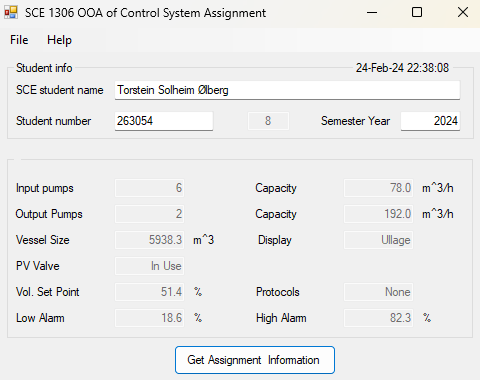
\includegraphics[width=12.6cm, height=8cm]{Assignment parameters.png}
\caption{The parameters for the buffer tank system. The system contains 6 input pumps and 2 output pumps, each with a set capacity. The Pressure Vacuume valve is present, and the display for the liquid level is set to ullage.}
\label{im:params}
		\end{figure}
In figure \ref{im:params} the parameters determined by the SCE 1319 OOA of Control System Assignment application \cite{task_params_app} for this project are presented, and these are used as specification for the project as well. \\
In this article an analysis of the project, using the Elaboration and Construction phase of the Unified Process \cite{lecture_notes}, the UP, will be performed. First the requirements will be extracted from the specification and a requirement document will be created. Then a use case diagram will be created from the functional requirements. Then a domain model will be created based on the specifications. Afterwards, a fully dressed use case document, or a FDUCD, will be created for the most important use case in the control system. Then a system sequence diagram will be created from the use case document, and finally a description of the future of the project with an estimate of how it could be solved will be provided.

	\section{Results}
		\subsection{Requirements}
The requirement document, found at the GitHub repository of the project \cite{github} and underneath this paragraph, contains a list of the requirements for the buffer tank control system. It follows the FURPS+ pattern and outlines both the functional and non-functional requirements. In short, it states that the control system needs to be able to control a set of input pumps and monitor the activities of a set of output pumps. It also needs to interact with a used, getting a desired level for the amount of liquid in the tank, and displaying alarms to the user. The document also outlines in what events the control system needs to output alarms, how to output them, and that it needs to control a safety PV valve to not risk to high pressure. Finally, it outlines the number of input and output pumps it needs to control and that there can't be any more devices in the buffer tank system than those specified in the specification. \\
\lstinputlisting{Requirement Document.txt}

		\subsection{Use Case Diagram}
The use case diagram, which can also be found at the GitHub repository \cite{github}, is a graphical representation of the functional requirements, with the system and its use cases linked with the different actors it needs to interact with. These actors are the user of the control system, the input pumps and the output pumps, and the PV valve. The use cases for the system, represented in the use case diagram, are controlling the input pumps, handle variations in time of the input and output, monitoring the output pumps, control the PV valve, set ideal liquid value, display current liquid value and display alarms.
			\begin{figure}[H]
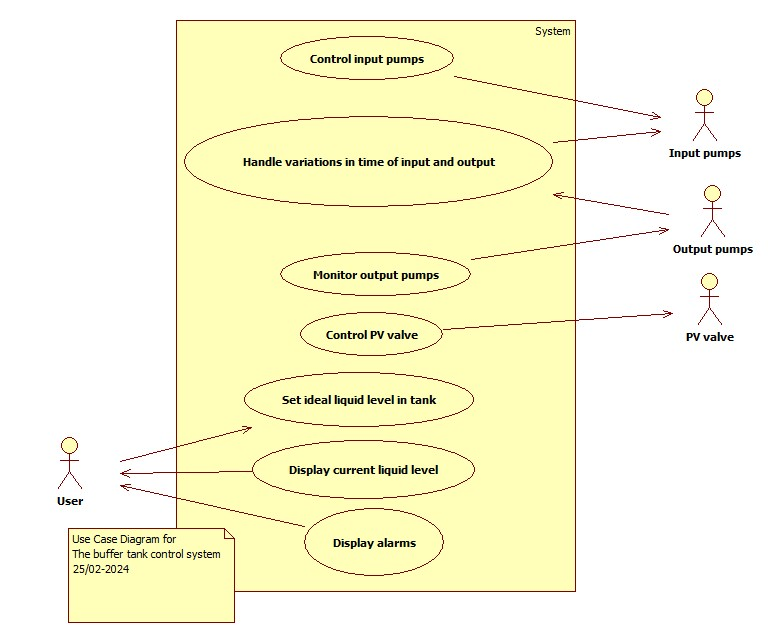
\includegraphics[width=12cm, height=12cm]{UseCaseDiagram.jpg}
\caption{The use case diagram for the control system. The actors are displayed, linked to the different use cases of the system which they interact with.}
\label{im:UCD}
			\end{figure}
The full use case diagram is displayed in figure \ref{im:UCD}.

		\subsection{Domain Model}
A domain model was created from the specification, and can also be found at the GitHub repository or seen in figure \ref{im:DM}.
			\begin{figure}[H]
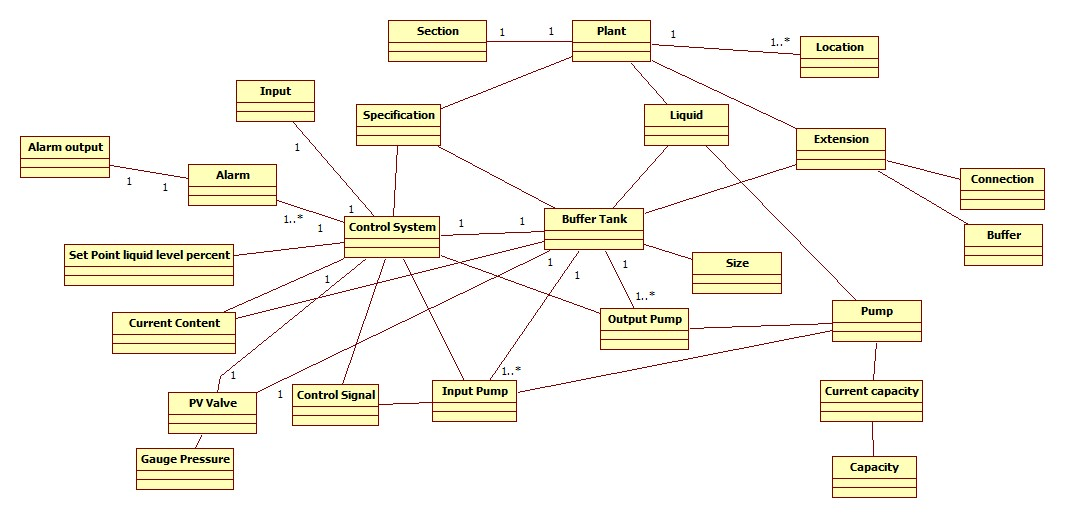
\includegraphics[width=12.8cm, height=8cm]{Domain Model.jpg}
\caption{The Domain model for the project containing all the items specified in the specification, with links to indicate how they interact with each other.}
\label{im:DM}
			\end{figure}
The diagram displays all the items specified in the specification, and also how they interact with each other. The control system and the buffer tank are particularly involved, with a lot of other items interacting or being linked to them. Some of the items also have multiplicity markings displaying if there are one or multiple of them present in the system.

		\subsection{Fully Dressed Use Case Document of the Most Important Use Case}
The FDUCD, found under this paragraph, outlines the full interaction between the input pumps and the control system when the control system controls the input pumps. This use case was chosen as the most important use case since it is directly responsible for the function of the system. With only this use case, and some preset configuration of the system, the system would be able to work. \\
The document mainly describes the normal scenario of the use case. This is the control system getting data from the pumps and itself, using that data to calculate a new input pump setting and sending that info to the input pumps. It also describes the different alternate routes which can be taken if any errors occur, like the lose of connection between pumps and control system, or the pumps extrema settings being inadequate in dealing with the current situation. \\
\lstinputlisting{Use Case Document.txt}
		
		\subsection{System Sequence Diagram of the FDUCD}
The system sequence diagram, found at the GitHub repository and also in figure \ref{im:SSD}, displays the time order of the FDUCD in a graphical way. The diagram includes two actors and one object, where the actors are the two types of pumps and the object is the control system. The sequence then starts with handling the collection of data, follows up with the calculation of new pump settings, and finishes with the transfer of the new settings and the check that these new settings where implemented correctly. The whole sequence is encapsulated in a loop, which indicates it is performed again and again.
			\begin{figure}[H]
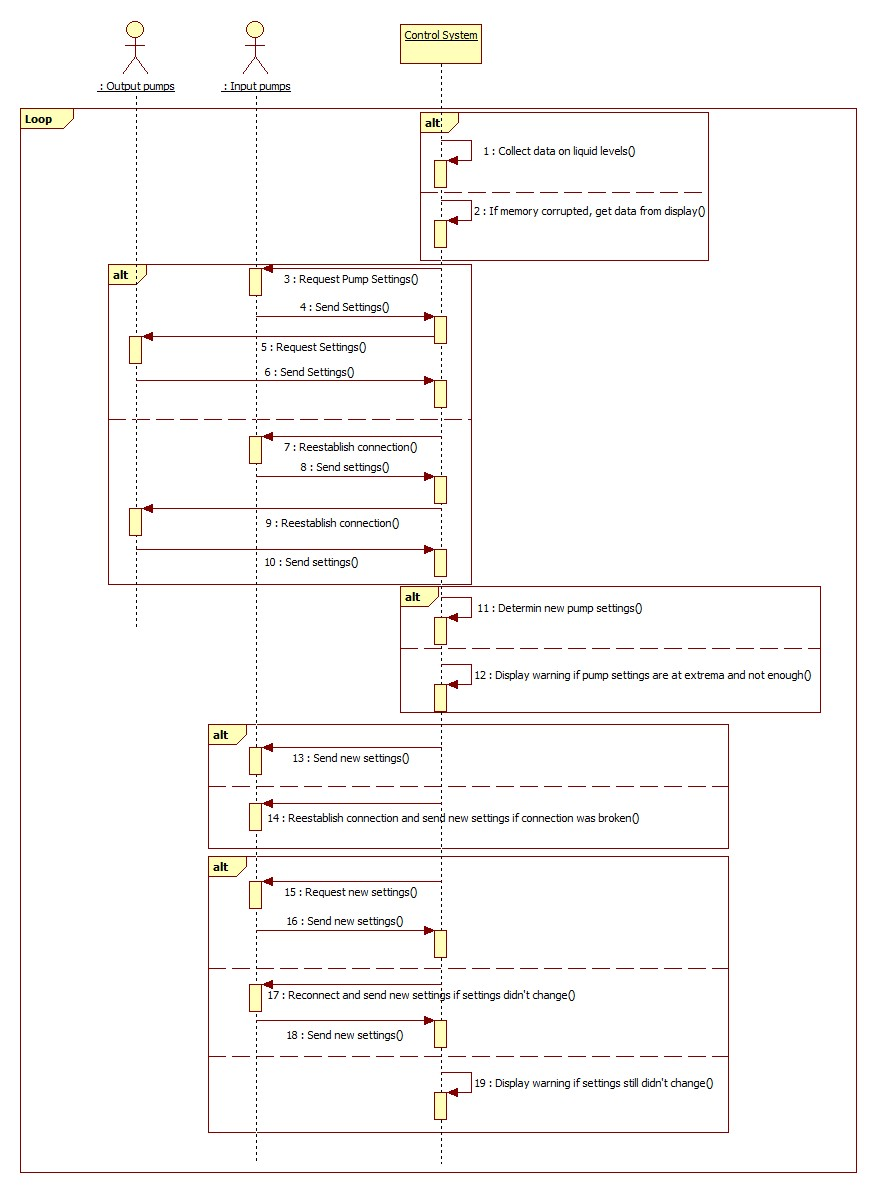
\includegraphics[width=12.8cm, height=15cm]{SequenceDiagram.jpg}
\caption{System sequence diagram for the most important use case, based on its FDUCD. There are two actors and one object, each of which perform a set of tasks and handles errors.}
\label{im:SSD}
			\end{figure}
	
	\section{Discussion}
		\subsection{Future of the Project (Development Process)}
			\subsubsection{Using the Unified Process to develop the control system}
Now that the broad documentation for how the system should be set up is almost finished, the next step would be to construct a working setup for the software based on the most important use case. Then, when this software has been developed and tested, the same process repeats itself. The the second most important use case is selected and development of it's documentation and software is performed, and then the third. Finally, when all the use cases have been handled the control system has been finished and it is ready to be deployed. Then the system is monitored and any unexpected problems or improvements are performed as they appear.
			
			\subsubsection{Relation between the tasks and the phases of the UP}
The different results outlined in this article are each connected to one of the two middle phases of the UP. First, the collection of requirements from the specification belongs to the Elaboration phase, as this is the planning and general design phase, and requirements are needed to design the general outlay of the system. Then, the construction of the use case diagram also belongs to the Elaboration phase, as this is only a graphical representation of some of the requirements. The Domain model is also part of the same phase as it is the first step in design of the object build up of the system. Then the selection of use cases, in this articles case only one, and construction of a FDUCD and system sequence diagram belongs to the Construction phase of the UP. This is because these are the first steps in the iterative process of constructing the solutions to each of the use case, and since UP is use case driven, they need to be done in the same iteration as the actual construction of the solution.
			
			\subsubsection{Usefulness in testing}
For later parts of the project, when testing the developed software, it is important to refer back to the requirements and the FDUCD as these express what the software must be capable of handling, and also how a success should be achieved.

			\subsubsection{Remaining time of the project}
Since the rest of the steps for finishing the project have been outlined, and the Elaboration phase has been finished, it is useful to estimate the time it would take for a finished project. This would be very useful when determining if the project is to continue to the next phase and also when the project can be expected to be finished. \\
Using the information available to us for this estimate, the size of the project and the availability of the team responsible for developing the control system, it is possible to make this. As this development is likely to fall to the team consisting only of the author of this project, a team size of one is assumed. Firstly, based on experience with the chosen teams earlier development time for similar systems, and the limited availability in the coming months, this development should at least take a week per use case. Summing the 7 remaining use cases, outlined in the use case diagram, together and adding equally as much time for the finale Transition phase the total time ends up at 8 weeks. Adding some time for unexpected problems, the remaining time of the project is two months.

	\section{Conclusion}
In the article, the project of developing a control system for a buffer tank has been outlined. The steps in the Elaboration phase and the first steps in a single iteration of the construction phase, of the UP, have been performed, and the results are a set of documentations and resources useful for later steps in the process. Finally, some speculation on the next steps in the project, the use case driven iterative part of the UP, and the time it will take to perform these steps have been presented. Based on this time, the project will be finished in about two months.

\clearpage

\printbibliography

\end{document}